\documentclass{article}
\usepackage{amsmath}
\usepackage{amssymb}
\usepackage{amsfonts}
\usepackage{graphicx} % Required for inserting images
\usepackage{float} % for [H] placement if needed
\title{Dynamic hedging}
% \author{Sathvika Miryala}
% \date{May 2026}

\begin{document}

\maketitle

\section{Introduction}

Options are fundamental instruments in modern financial markets, widely used for hedging, speculation, and risk management. A central problem in quantitative finance is the effective management of option risk through dynamic hedging strategies. The classical Black--Scholes--Merton framework provides a theoretical foundation for this problem, demonstrating that, under idealized assumptions, a derivative can be perfectly replicated through continuous-time trading in the underlying asset and a risk-free bond.

However, these assumptions are rarely satisfied in practice. Real-world markets impose discrete trading intervals, transaction costs, and time-varying volatility. As a result, perfect replication is unattainable, and hedging strategies inevitably incur tracking error. Understanding the sources and magnitude of this error is critical for both theoretical insight and practical implementation.

This study aims to bridge the gap between continuous-time financial theory and discrete-time market reality by developing a comprehensive dynamic hedging framework for European options. The framework enables systematic evaluation of hedging performance under realistic conditions, incorporating discrete rebalancing, transaction costs, and empirical market data.

The core objectives of this work are threefold. First, we construct a backtesting engine that implements self-financing delta-hedging strategies using Black--Scholes sensitivities. Second, we quantify hedging performance across different rebalancing frequencies and benchmark strategies, including no-hedge and static hedge baselines. Third, we analyze the sources of hedging error through both theoretical and empirical lenses, with particular emphasis on discretization effects and model misspecification.

To interpret the observed replication error, two complementary analytical tools are employed. The Bertsimas--Kogan--Lo (BKL) approximation provides a theoretical benchmark for the variance induced purely by discrete rebalancing. In parallel, a Greek-based P\&L attribution framework decomposes realized hedging outcomes into contributions from Delta, Gamma, Theta, and Vega, allowing for a detailed diagnosis of underlying risk drivers.

Beyond measurement, the study also addresses optimization. Rather than minimizing variance alone, hedging strategies are evaluated using Conditional Value at Risk (CVaR), a coherent risk measure that captures extreme downside outcomes. This enables a principled trade-off between replication accuracy and transaction costs, leading to the identification of economically optimal rebalancing frequencies.

Finally, the framework is extended to a real-world setting using market data, where key theoretical assumptions—particularly constant volatility—are relaxed. A dedicated volatility mismatch experiment isolates the impact of incorrect volatility estimation, highlighting the role of model risk in dynamic hedging.

The findings of this study demonstrate that while the Black--Scholes model provides an essential theoretical benchmark, real-world hedging performance is driven by a complex interplay of discretization effects, transaction costs, and volatility dynamics. These results offer practical insights for the design of robust hedging strategies and contribute to a deeper understanding of the limitations of classical financial models.
\section{Background}
\subsection{ Conditional Value at Risk (CVar)}

To quantify tail risk in the dynamic hedging strategy, we employ CVaR, also known as \emph{Expected Shortfall} (ES). Unlike Value at Risk (VaR), which does not satisfy the subadditivity property and is therefore not a coherent risk measure, CVaR provides a mathematically consistent and robust characterization of extreme losses. This makes it particularly suitable for evaluating the risk of discrete hedging strategies, where large deviations may arise due to market frictions and rebalancing constraints.

Let $L$ denote a continuous random variable representing the loss of the delta-hedging portfolio. Specifically, we define the loss as the negative hedging error:
\[
L = - \big( V_{\text{portfolio}} - V_{\text{option}} \big),
\]
where $V_{\text{portfolio}}$ is the value of the replicating portfolio and $V_{\text{option}}$ is the theoretical option price.

Let $(\Omega, \mathcal{F}, \mathbb{P})$ be a probability space and let $F_L(l) = \mathbb{P}(L \leq l)$ denote the cumulative distribution function (CDF) of $L$.

For a confidence level $\alpha \in (0,1)$ (commonly $\alpha = 0.95$ or $0.99$), the Value at Risk is defined as the $\alpha$-quantile of the loss distribution:
\[
\text{VaR}_\alpha(L) = \inf \{ l \in \mathbb{R} \mid F_L(l) \geq \alpha \}.
\]

The Conditional Value at Risk is defined as the expected loss conditional on exceeding the VaR threshold. For continuous distributions:
\[
\text{CVaR}_\alpha(L) = \mathbb{E} \left[ L \mid L \geq \text{VaR}_\alpha(L) \right].
\]

% An equivalent and more general formulation of CVaR expresses it as the average of the upper tail of the VaR curve:
% \[
% \text{CVaR}_\alpha(L) = \frac{1}{1 - \alpha} \int_{\alpha}^{1} \text{VaR}_\gamma(L) \, d\gamma.
% \]

% If $L$ admits a continuous density function $f_L(l)$, this reduces to a tail expectation:
% \[
% \text{CVaR}_\alpha(L) = \frac{1}{1 - \alpha} 
% \int_{\text{VaR}_\alpha(L)}^{\infty} l \, f_L(l) \, dl.
% \]

In a continuous-time setting, perfect replication is theoretically achievable under ideal assumptions. However, in practice, hedging occurs at discrete intervals $\Delta t$, introducing tracking error and transaction costs.

To balance tail risk against trading costs, we define the following objective function:
\[
J(\Delta t) = \max\Big(0, \, \text{CVaR}_\alpha\big(L(\Delta t)\big)\Big) 
+ \mathbb{E}\big[\text{TC}(\Delta t)\big],
\]
where $\text{TC}(\Delta t)$ denotes the cumulative transaction costs associated with the hedging strategy.

This formulation penalizes extreme losses through CVaR while incorporating the economic cost of rebalancing. As a result, it provides a tractable and convex framework for determining an optimal hedging frequency that balances risk reduction against market frictions.

\subsection{The Bertsimas--Kogan--Lo (BKL) }

The classical BlackScholes framework assumes continuous-time trading, under which a derivative can be perfectly replicated by dynamically adjusting a self-financing portfolio. In this idealized setting, continuous rebalancing ($\Delta t \to 0$) ensures that the replication error is identically zero.

In practice, however, trading occurs at discrete time intervals. This introduces \emph{discretization error}, as the hedging portfolio is only updated intermittently while the underlying asset evolves continuously. BKL framework provides a quantitative approximation of the variance of this unavoidable hedging error.
Delta hedging neutralizes the first-order sensitivity of the option price with respect to the underlying asset. However, the option remains exposed to its second-order sensitivity, known as Gamma ($\Gamma$). 
Between rebalancing times, the underlying asset price changes randomly, and the linear hedging portfolio cannot capture the curvature of the option payoff. This mismatch generates a residual tracking error, which the BKL approximation characterizes.

Let $S_t$ denote the underlying asset price following a geometric Brownian motion with volatility $\sigma$, and let $V(t,S_t)$ denote the option price. Over a small time interval $\Delta t$, a second-order expansion yields:
\[
\Delta V_t \approx \Theta_t \Delta t + \Delta_t \Delta S_t + \frac{1}{2} \Gamma_t (\Delta S_t)^2.
\]

A delta-hedged portfolio eliminates the linear term $\Delta_t \Delta S_t$, leaving a residual error driven by Gamma. Using the BlackScholes partial differential equation to simplify terms, the one-step hedging error can be approximated as:
\[
e_t \approx \frac{1}{2} \Gamma_t \left[ (\Delta S_t)^2 - \sigma^2 S_t^2 \Delta t \right].
\]

Expressing the stock increment in terms of a Wiener process ($\Delta W_t$), this becomes:
\[
e_t \approx \frac{1}{2} \sigma^2 S_t^2 \Gamma_t \left( (\Delta W_t)^2 - \Delta t \right).
\]

Although the expected value of the local error is zero, its variance is strictly positive. The BKL approximation shows that the variance of the single-step hedging error is:
\[
\text{Var}(e_t) = \frac{1}{2} \left( \sigma^2 S_t^2 \Gamma_t \right)^2 (\Delta t)^2.
\]

Aggregating over $N$ discrete rebalancing intervals up to maturity $T$, the total hedging error variance is approximated by:
\[
\text{Var}_{\text{Total}} \approx \sum_{i=1}^{N} 
\frac{1}{2} \left( \sigma^2 S_{t_i}^2 \Gamma_{t_i} \right)^2 (\Delta t)^2.
\]

The BKL result provides a crucial extension of the Black--Scholes model by explicitly quantifying the impact of discrete trading. While Black--Scholes guarantees perfect replication in continuous time, BKL demonstrates that in realistic settings, hedging error is:

\begin{itemize}
    \item \textbf{Unavoidable:} It arises purely from discrete-time trading constraints.
    \item \textbf{Gamma-driven:} Higher curvature leads to larger replication error.
    \item \textbf{Frequency-dependent:} The error decreases quadratically as $\Delta t \to 0$.
\end{itemize}

This quadratic scaling formally justifies the convergence of discrete hedging to the continuous-time ideal.

% \subsection{Relevance for Empirical Hedging}

% In practical implementations, the BKL approximation serves as a theoretical benchmark for hedging performance. By comparing the empirically observed variance of hedging P\&L with the BKL prediction across different rebalancing frequencies, one can verify whether deviations are due to model limitations or execution inefficiencies.

% Thus, the BKL framework bridges the gap between the idealized Black--Scholes model and real-world trading, providing a rigorous foundation for analyzing and optimizing discrete hedging strategies.
\section{Experimental details}
This study develops a dynamic, self-financing delta-hedging simulation framework for European options under discrete trading constraints. The objective is to quantify replication error, attribute its sources, and evaluate optimal hedging frequency under transaction costs and tail-risk considerations.

The framework is implemented across two environments:
(i) a synthetic Black--Scholes benchmark for theoretical validation, and 
(ii) a real-market pipeline using historical data and option chains sourced from Yahoo Finance.

\subsection{Data Environments}

\subsubsection{Synthetic Baseline}

The baseline experiment isolates discrete hedging error in a controlled setting consistent with the Black--Scholes--Merton (BSM) model.

\begin{itemize}
    \item \textbf{Underlying:} Synthetic SPY price process
    \item \textbf{Period:} January 1, 2020 -- December 31, 2024
    \item \textbf{Initial Maturity:} $T = 21$ trading days
    \item \textbf{Volatility:} $\sigma = 0.20$
    \item \textbf{Risk-free rate:} $r = 0.02$
    \item \textbf{Dividend yield:} $q = 0$
    \item \textbf{Transaction cost:} 5 basis points per trade
\end{itemize}

This environment ensures that any observed replication error arises solely from discrete rebalancing.

\subsubsection{Empirical Market Data (Yahoo Finance)}

The empirical framework integrates real historical prices and option chains.

\paragraph{Option Selection Criteria}
\begin{itemize}
    \item \textbf{Maturity constraint:} $\geq 30$ days to expiration
    \item \textbf{Moneyness filter:} strike within $\pm 10\%$ of spot
    \item \textbf{Delta targeting:} $|\Delta| \in [0.25, 0.75]$, centered near $0.5$
    \item \textbf{Liquidity filter:} strictly positive open interest
\end{itemize}

\paragraph{Volatility Handling}
If implied volatility is unavailable or below a threshold ($0.05$), it is replaced with a 21-day rolling realized volatility estimate, bounded below to ensure numerical stability.

\paragraph{Data Alignment}
Option and underlying time series are synchronized via an inner join on daily timestamps. Time-to-maturity is computed as a fraction of calendar time:
\[
\tau = \frac{T - t}{365}.
\]

\subsection{Option Pricing and Greeks}

All option valuations and sensitivities are computed under the Black--Scholes framework with continuous dividend yield:
\[
d_1 = \frac{\ln(S/K) + (r - q + \frac{1}{2}\sigma^2)\tau}{\sigma\sqrt{\tau}}, 
\quad
d_2 = d_1 - \sigma\sqrt{\tau}.
\]

Key sensitivities used in the hedging engine include:
\begin{itemize}
    \item Delta: $\Delta = e^{-q\tau}\Phi(d_1)$
    \item Gamma: $\Gamma = \frac{e^{-q\tau}\phi(d_1)}{S\sigma\sqrt{\tau}}$
    \item Vega and Theta for attribution analysis
\end{itemize}

\subsection{Hedging Strategy and Portfolio Dynamics}

The replication strategy assumes a self-financing portfolio consisting of the underlying asset and a cash account.

\paragraph{Initial Condition}
The strategy is implemented from the perspective of an option writer:
\[
\text{Cash}_0 = V_{\text{option}}(t_0).
\]

\paragraph{Rebalancing Rule}
At each rebalancing time, the target position is:
\[
\Delta_{\text{target}} = \Delta_t.
\]

The number of shares traded is:
\[
|\Delta_{\text{target}} - \Delta_{\text{current}}|.
\]

\paragraph{Transaction Costs}
Each trade incurs proportional costs:
\[
\text{TC} = |\text{Shares Traded}| \times S_t \times 0.0005.
\]

\paragraph{Cash Dynamics}
The cash account evolves according to:
\[
\text{Cash}_t = \text{Cash}_{t-1} e^{r\Delta t} - (\text{Trade Value} + \text{TC}).
\]

\subsection{Rebalancing Strategies}

The following strategies are evaluated:

\begin{itemize}
    \item \textbf{Periodic Hedging:} Rebalancing every 1, 2, or 5 trading days
    \item \textbf{Static Hedge:} Initial delta held constant until maturity
    \item \textbf{No Hedge:} Pure option exposure without replication
    \item \textbf{Continuous Benchmark:} Idealized zero-error reference
\end{itemize}

\subsection{Replication Error and Risk Metrics}

\paragraph{Hedging Error}
Replication performance is evaluated via:
\[
L_t = V_{\text{portfolio},t} - V_{\text{option},t}.
\]

\paragraph{BKL Variance Benchmark}
The discrete hedging error is compared against the Bertsimas--Kogan--Lo approximation:
\[
\text{Var}(e_t) \approx \frac{1}{2} \left( \sigma^2 S_t^2 \Gamma_t \right)^2 (\Delta t)^2.
\]

This provides a theoretical lower bound on achievable hedging accuracy under discrete trading.

\paragraph{Tail Risk Measures}
\begin{itemize}
    \item Value at Risk (VaR)
    \item Conditional Value at Risk (CVaR):
    \[
    \text{CVaR}_\alpha = \mathbb{E}[L \mid L \geq \text{VaR}_\alpha]
    \]
\end{itemize}

\subsection{P\&L Attribution}

To diagnose sources of hedging error, the total P\&L is decomposed into Greek components:
\[
\Delta \text{PnL}_{\Delta} = \Delta_{t-1}(S_t - S_{t-1}),
\]
\[
\Delta \text{PnL}_{\Gamma} = \frac{1}{2}\Gamma_{t-1}(S_t - S_{t-1})^2,
\]
\[
\Delta \text{PnL}_{\Theta} = \Theta_{t-1}(\tau_{t-1} - \tau_t),
\]
\[
\Delta \text{PnL}_{\mathcal{V}} = \mathcal{V}_{t-1}(\sigma_t - \sigma_{t-1}).
\]

This decomposition enables identification of whether deviations arise from time decay, volatility shocks, or discrete hedging effects.

\subsection{Optimization Objective}

To determine the optimal hedging frequency, strategies are evaluated using a convex objective function combining tail risk and transaction costs:
\[
J(\Delta t) = \max(0, -\text{CVaR}_{95}) + \sum \text{Transaction Costs}.
\]

This formulation prioritizes minimizing extreme downside risk while penalizing excessive trading, thereby balancing hedging precision against market frictions.
\subsection{Volatility Mismatch Experiment}

\subsubsection{Motivation}

The Black--Scholes framework assumes constant volatility, an assumption that is systematically violated in real financial markets. In practice, discrepancies between the volatility used for pricing and hedging (implied volatility) and the volatility realized by the underlying asset lead to persistent hedging errors.

To isolate and quantify the impact of volatility misspecification, a dedicated volatility mismatch experiment is conducted. This experiment evaluates the extent to which incorrect volatility assumptions alone generate replication error, independent of discrete rebalancing effects.

\subsubsection{Experimental Design}

The experiment is implemented by simulating two parallel hedging strategies on an identical underlying price path. All parameters are held constant except for the volatility input used in the Black--Scholes pricing and Greek calculations.

\paragraph{Configuration}
\begin{itemize}
    \item \textbf{Underlying:} SPY
    \item \textbf{Period:} January 1, 2020 -- December 31, 2024
    \item \textbf{Initial maturity:} $T = 21$ trading days
    \item \textbf{Rebalancing frequency:} Daily ($\Delta t = 1$)
    \item \textbf{Transaction cost:} 5 basis points
\end{itemize}

Daily rebalancing is enforced to eliminate discretization error, ensuring that observed deviations arise purely from volatility misspecification.

\subsubsection{Parallel Hedging Framework}

Two hedging environments are constructed:

\paragraph{Fixed Volatility Model}
The hedging strategy assumes a constant volatility:
\[
\sigma = 0.20.
\]
This value is used for both option pricing and Greek computation throughout the simulation, regardless of market conditions.

\paragraph{Realized Volatility Model}
The hedging strategy updates volatility dynamically using a rolling estimate of realized volatility:
\[
\sigma_t = \sqrt{252} \cdot \text{StdDev} \left( \ln \left( \frac{S_{t-i}}{S_{t-i-1}} \right) \right)_{i=1}^{21}.
\]

This produces a time-varying volatility input consistent with observed market fluctuations.

\paragraph{Warm-up Procedure}
To ensure numerical consistency, a 21-day warm-up window is applied prior to the start of the hedging period. This guarantees that the rolling volatility estimate is fully initialized and avoids missing data issues.

\subsubsection{Interpretation of Results}

Because both strategies operate on the same price path and rebalance daily, any divergence in replication performance is attributable solely to differences in volatility assumptions.

The resulting hedging error directly measures the cost of volatility misspecification.

Using the P\&L attribution framework, deviations can be decomposed into:

\begin{itemize}
    \item \textbf{Gamma-driven error:} Incorrect Delta due to misestimated volatility leads to suboptimal hedge ratios, amplifying curvature-related losses during price movements.
    \item \textbf{Vega exposure:} Differences in volatility inputs generate systematic pricing discrepancies, contributing to P\&L drift.
\end{itemize}

\subsubsection{Implications}

This experiment demonstrates that even under idealized conditions of continuous rebalancing, incorrect volatility assumptions introduce significant and persistent hedging error. 

It highlights a fundamental limitation of the Black--Scholes model: while discretization error can be reduced through more frequent trading, volatility misspecification constitutes an independent and irreducible source of model risk.

Consequently, accurate volatility estimation is critical for effective dynamic hedging, and models assuming constant volatility may perform poorly in non-stationary market environments.
The methodology integrates theoretical modeling, empirical data, and risk-based optimization into a unified framework. By benchmarking against both Black--Scholes and BKL predictions, the study rigorously evaluates the trade-off between hedging accuracy and implementation costs in realistic market settings.
\section{Results}

The performance of the dynamic delta-hedging framework is evaluated across two environments: a controlled synthetic Black--Scholes setting and an empirical implementation using real-world options data.

\subsection{Theoretical Baseline Results}

Under the Black--Scholes assumptions of constant volatility ($\sigma = 0.20$) and risk-free rate ($r = 0.02$), the hedging error behaves consistently with theoretical predictions.

The continuous-time benchmark yields zero replication error and zero transaction costs, confirming the validity of the implementation.

For discrete hedging strategies, the final absolute hedging error increases monotonically with rebalancing interval:
\begin{itemize}
    \item Daily hedging: $\$2.38$
    \item Every 2 days: $\$2.68$
    \item Weekly (5 days): $\$3.60$
\end{itemize}

Benchmark strategies exhibit significantly larger deviations:
\begin{itemize}
    \item No hedge: $\$6.61$
    \item Static hedge: $\$4.79$
\end{itemize}

When accounting for transaction costs, the optimal strategy selected via CVaR minimization is the 5-day rebalancing policy, which achieves the lowest combined risk-cost trade-off.

\subsection{Empirical Results Using Market Data}

In the empirical setting, an at-the-money SPY call option was analyzed using historical data. Due to unreliable implied volatility data, a 21-day rolling realized volatility estimator was employed.

The results deviate significantly from the theoretical baseline:
\begin{itemize}
    \item The unhedged position incurs a large loss ($-\$10.70$), reflecting directional exposure.
    \item Delta-hedged strategies generate large positive terminal values (e.g., $+\$31.30$ for daily hedging), indicating systematic over-hedging.
\end{itemize}

These outcomes demonstrate that model misspecification, particularly in volatility estimation, dominates discretization effects in real-world applications.

\subsection{Visualization of Hedging Dynamics}

\paragraph{Market Inputs and Delta Allocation}

Figure~\ref{fig:market_inputs} illustrates the evolution of the underlying asset price and option value relative to the strike, primarily demonstrating the option moving cleanly in-the-money in the synthetic model versus oscillating in the Yahoo empirical setup. Figure~\ref{fig:stock_shares} shows the corresponding hedge ratios. As the option moves in-the-money, the delta converges toward unity, while the static hedge remains fixed.

\begin{figure}[htbp]
    \centering
    \begin{minipage}{0.45\textwidth}
        \centering
        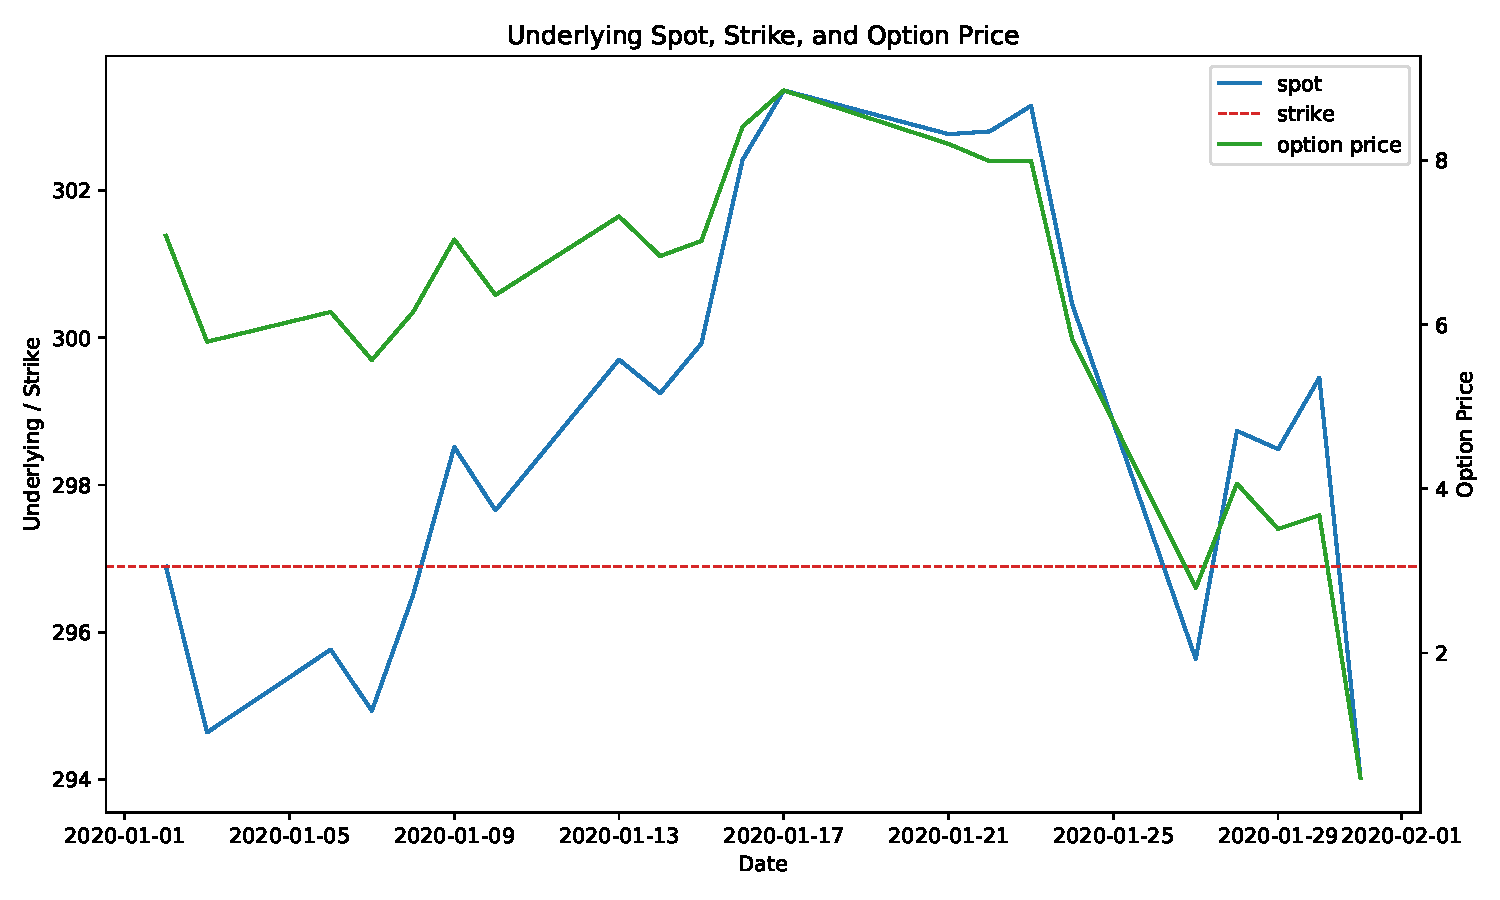
\includegraphics[width=\linewidth]{outputs/figures/market_inputs.pdf}
        \caption{Theoretical Synthetic Baseline: Underlying limits.}
        \label{fig:market_inputs_theo}
    \end{minipage}\hfill
    \begin{minipage}{0.45\textwidth}
        \centering
        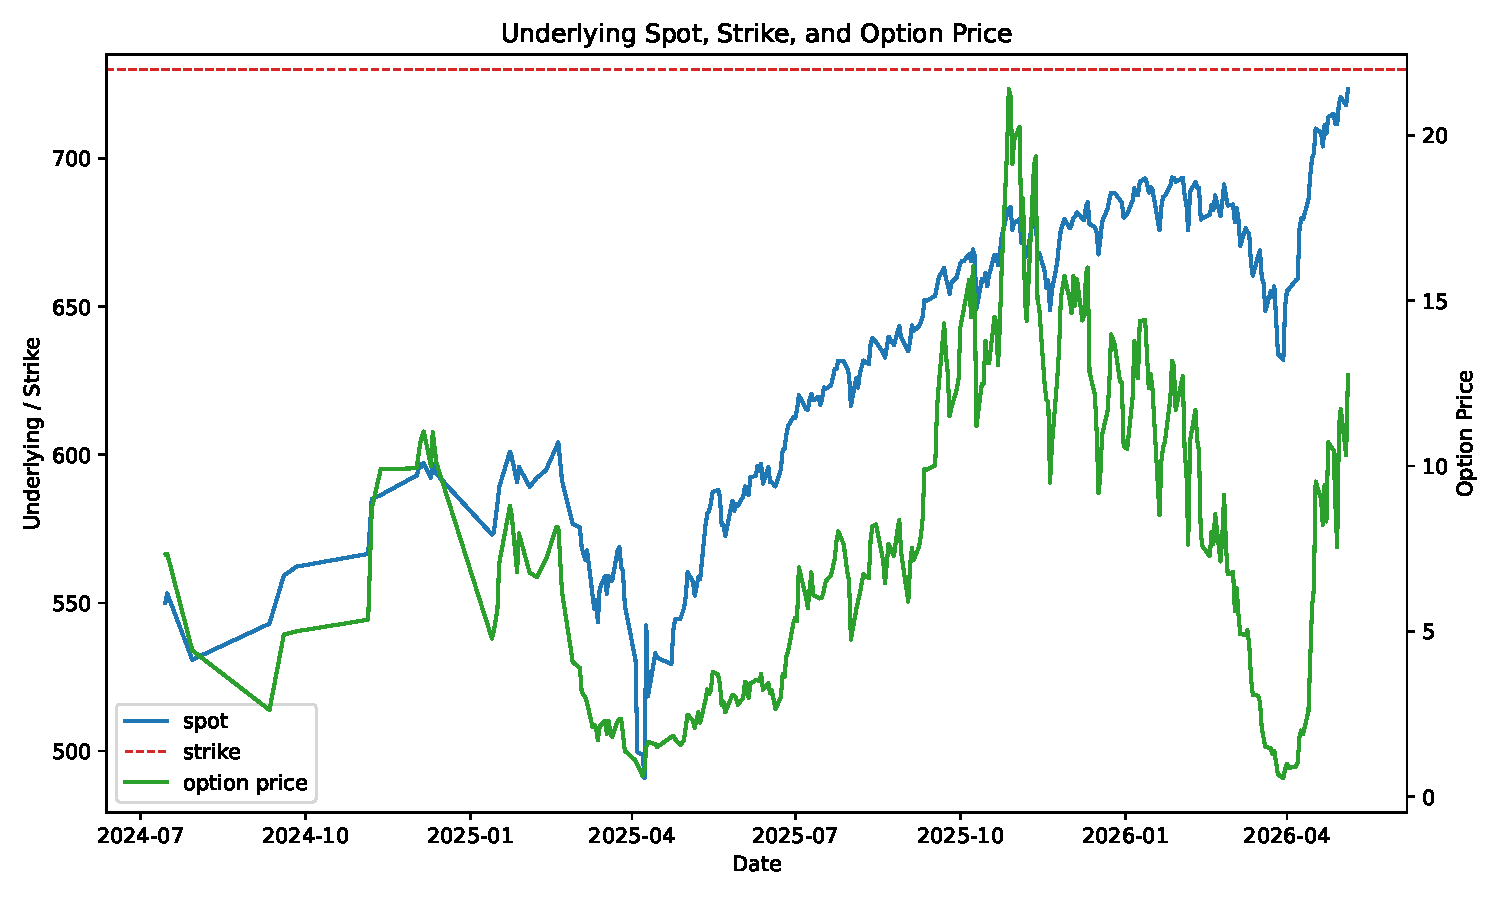
\includegraphics[width=\linewidth]{outputs/figures/yahoo_option/market_inputs.pdf}
        \caption{Empirical Yahoo Options: Observed market actions.}
        \label{fig:market_inputs_yahoo}
    \end{minipage}
\end{figure}

\begin{figure}[htbp]
    \centering
    \begin{minipage}{0.45\textwidth}
        \centering
        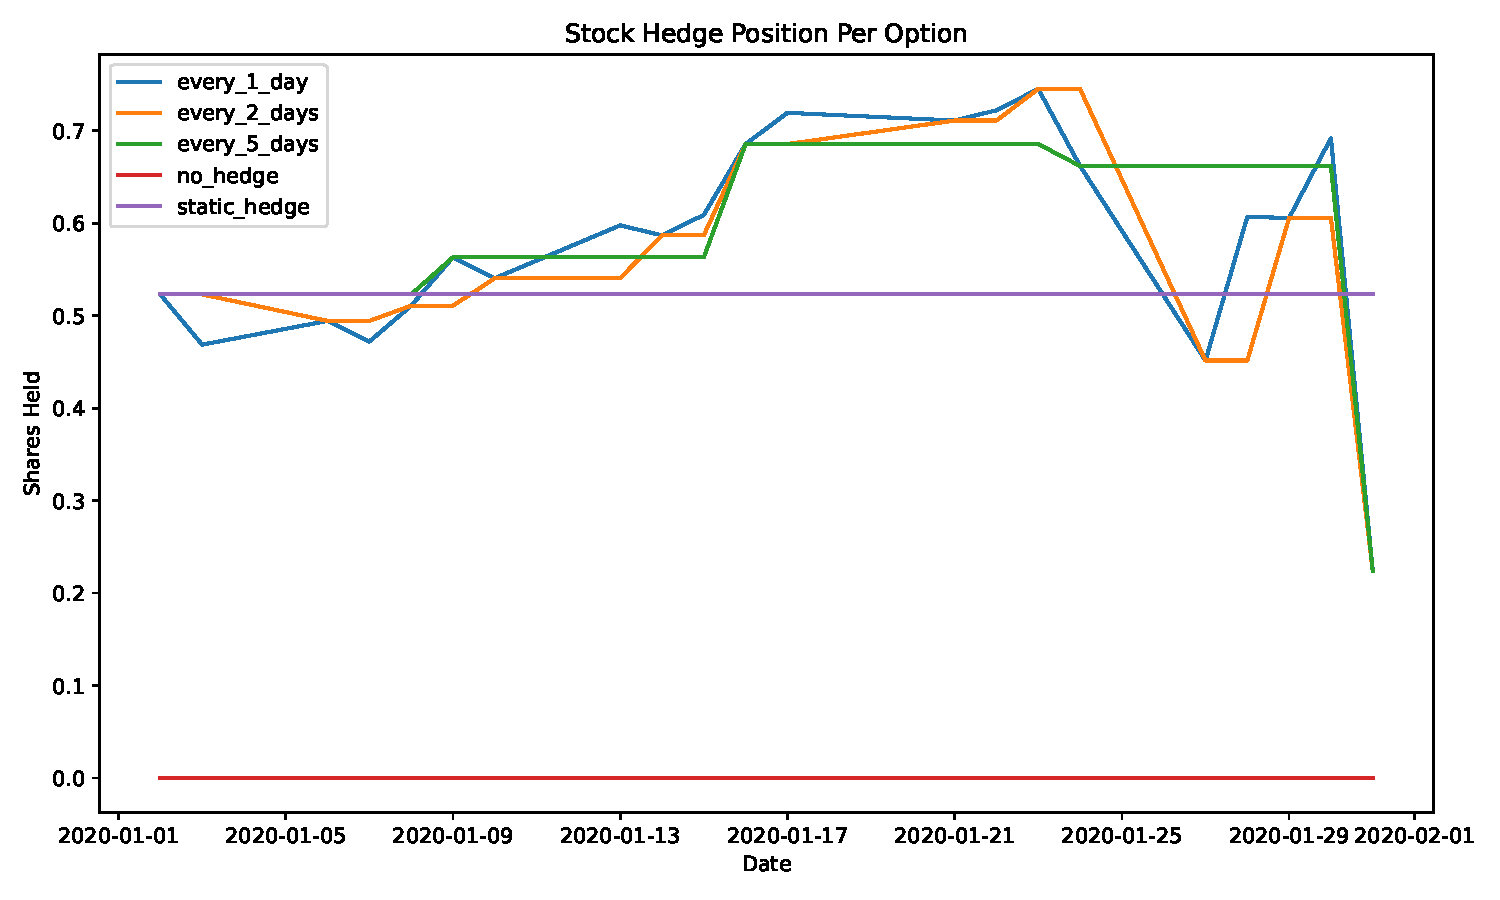
\includegraphics[width=\linewidth]{outputs/figures/stock_shares_paths.pdf}
        \caption{Theoretical Stock Shares: Smooth analytical Delta allocation limits.}
        \label{fig:stock_shares_theo}
    \end{minipage}\hfill
    \begin{minipage}{0.45\textwidth}
        \centering
        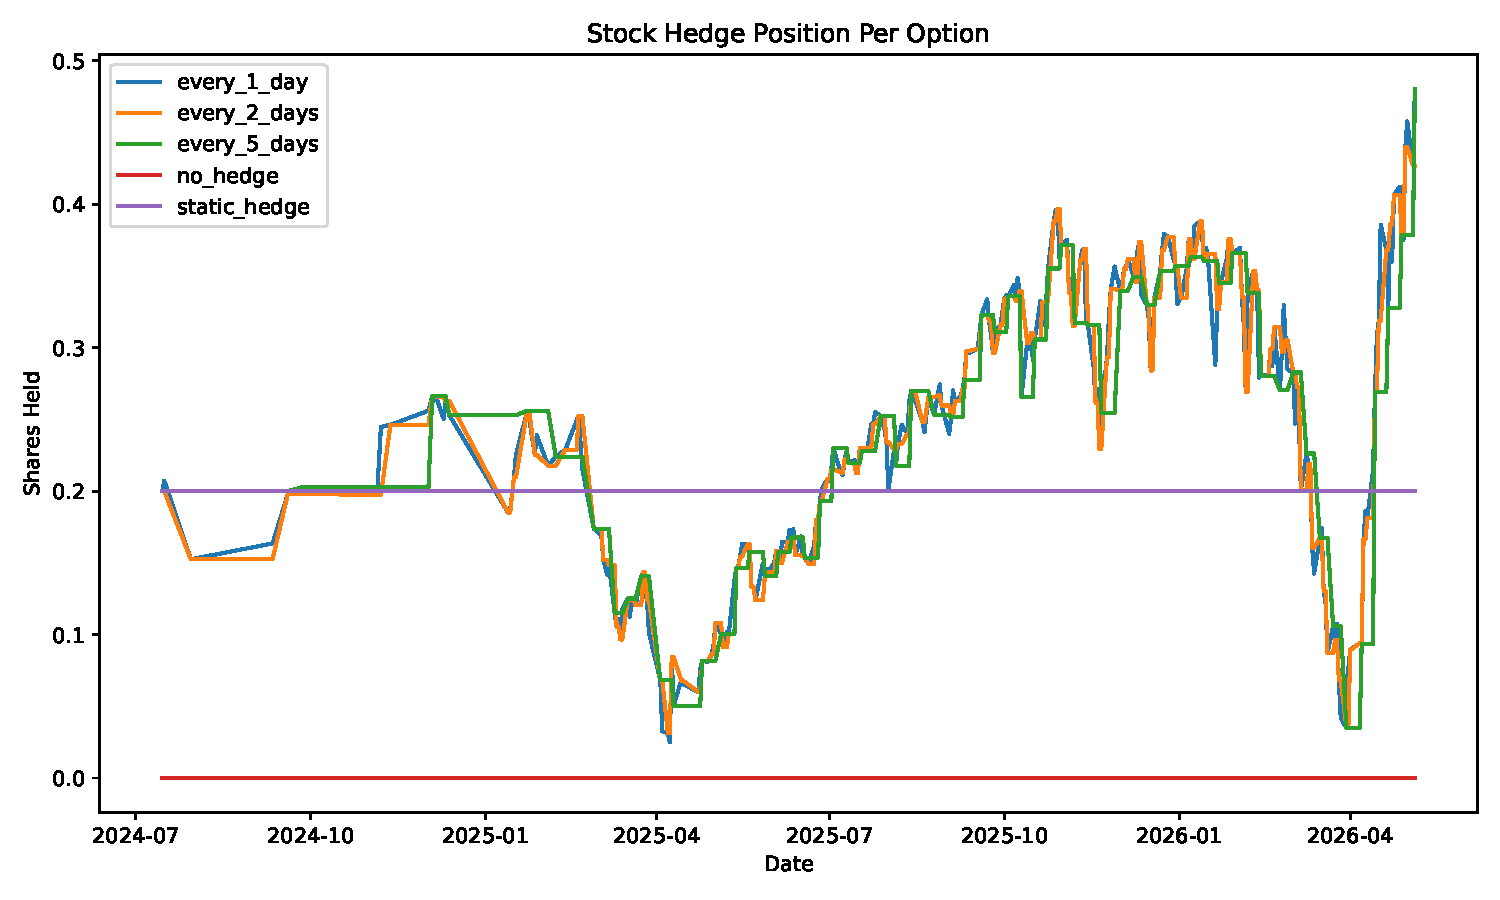
\includegraphics[width=\linewidth]{outputs/figures/yahoo_option/stock_shares_paths.pdf}
        \caption{Empirical Stock Shares: Erratic, reality-driven Delta limits.}
        \label{fig:stock_shares_yahoo}
    \end{minipage}
\end{figure}

\paragraph{Portfolio Value Evolution}

Figure~\ref{fig:portfolio_value} compares the replication portfolio value with the theoretical option price. In the synthetic case, trajectories closely track the option value. In contrast, empirical results exhibit large divergence due to volatility mismatch.

\begin{figure}[htbp]
    \centering
    \begin{minipage}{0.45\textwidth}
        \centering
        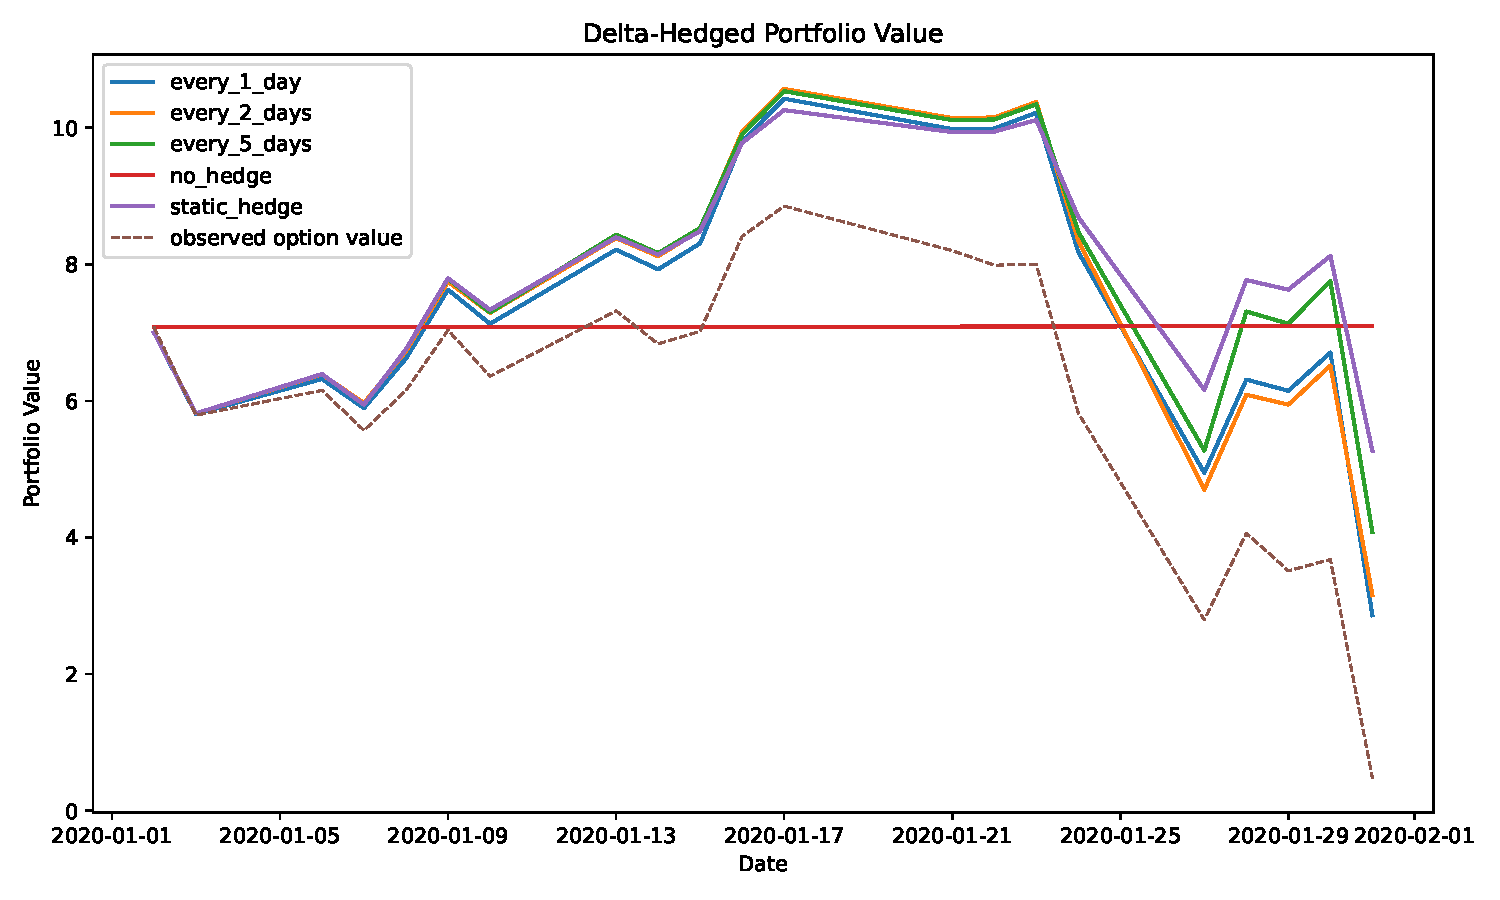
\includegraphics[width=\linewidth]{outputs/figures/portfolio_value_paths.pdf}
        \caption{Theoretical Baseline: Tight tracking of portfolio value to theoretical option value.}
        \label{fig:portfolio_theoretical}
    \end{minipage}\hfill
    \begin{minipage}{0.45\textwidth}
        \centering
        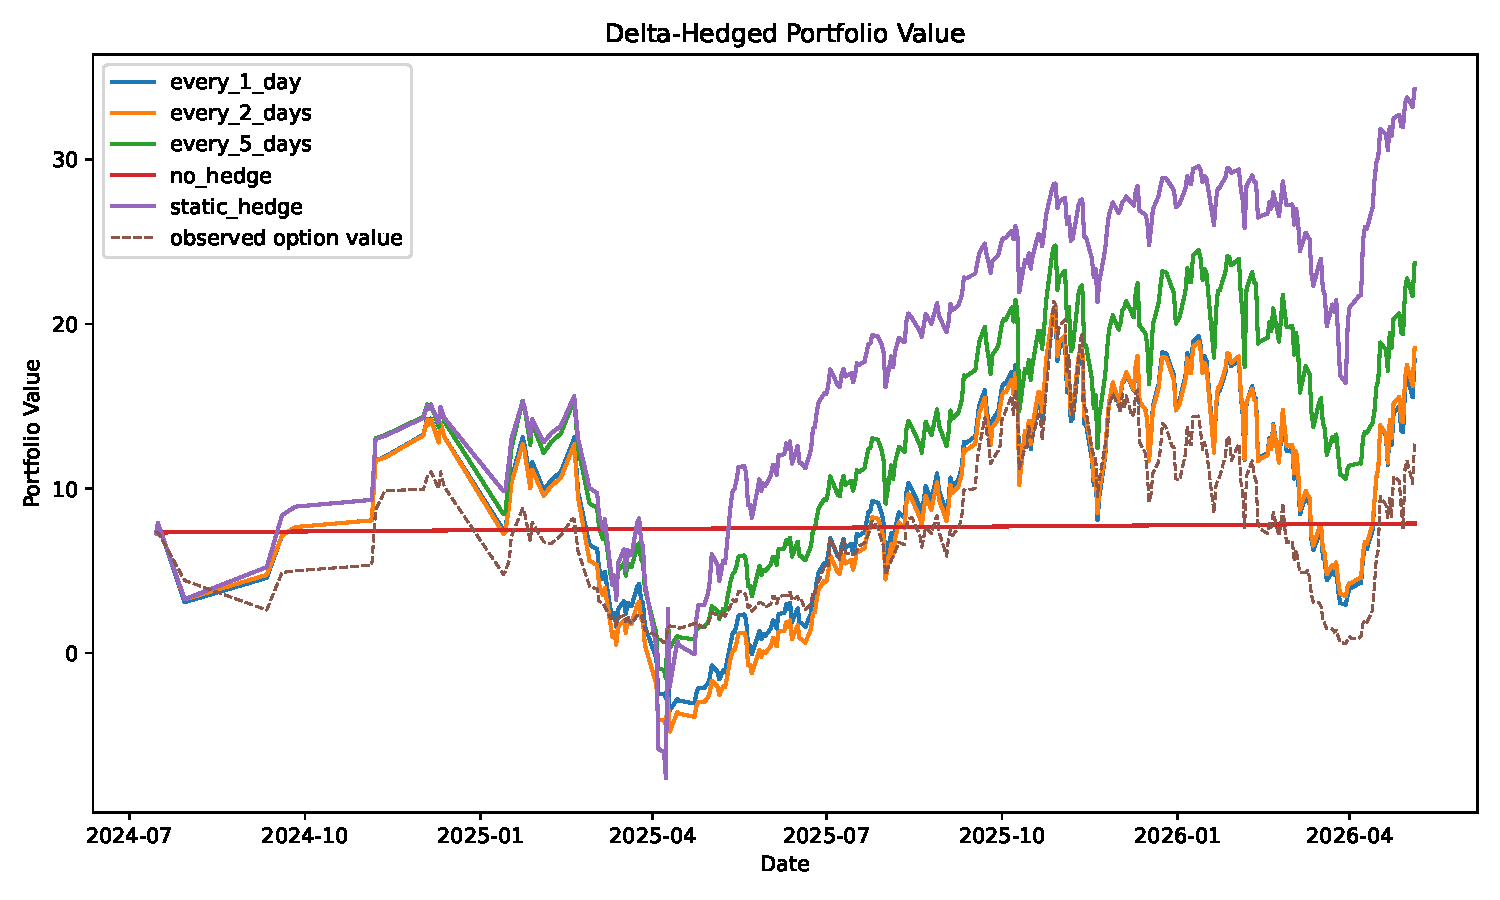
\includegraphics[width=\linewidth]{outputs/figures/yahoo_option/portfolio_value_paths.pdf}
        \caption{Empirical Yahoo Options: Severe divergence due to real-world volatility mismatch.}
        \label{fig:portfolio_yahoo}
    \end{minipage}
\end{figure}

\paragraph{Hedging Error Evolution}

Figure~\ref{fig:hedge_error_theoretical} shows the time evolution of hedging error, while Figure~\ref{fig:error_theoretical} summarizes terminal outcomes across theoretical and analytical spheres.

\begin{figure}[htbp]
    \centering
    \begin{minipage}{0.45\textwidth}
        \centering
        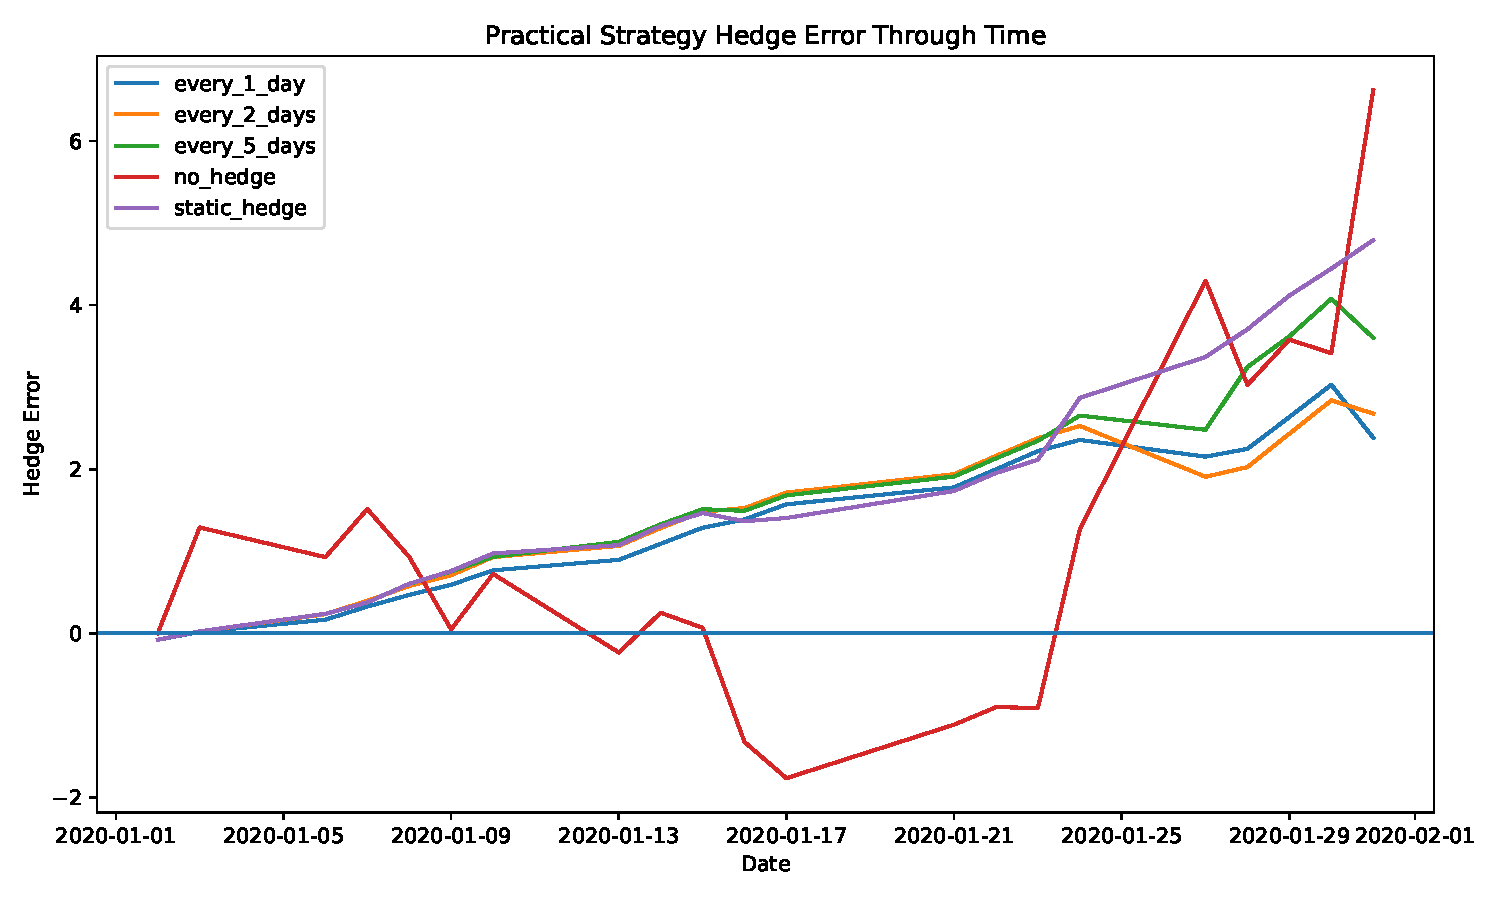
\includegraphics[width=\linewidth]{outputs/figures/hedge_error_paths.pdf}
        \caption{Theoretical Baseline: Smooth replication bleed surrounding zero constraint limits.}
        \label{fig:hedge_error_theoretical}
    \end{minipage}\hfill
    \begin{minipage}{0.45\textwidth}
        \centering
        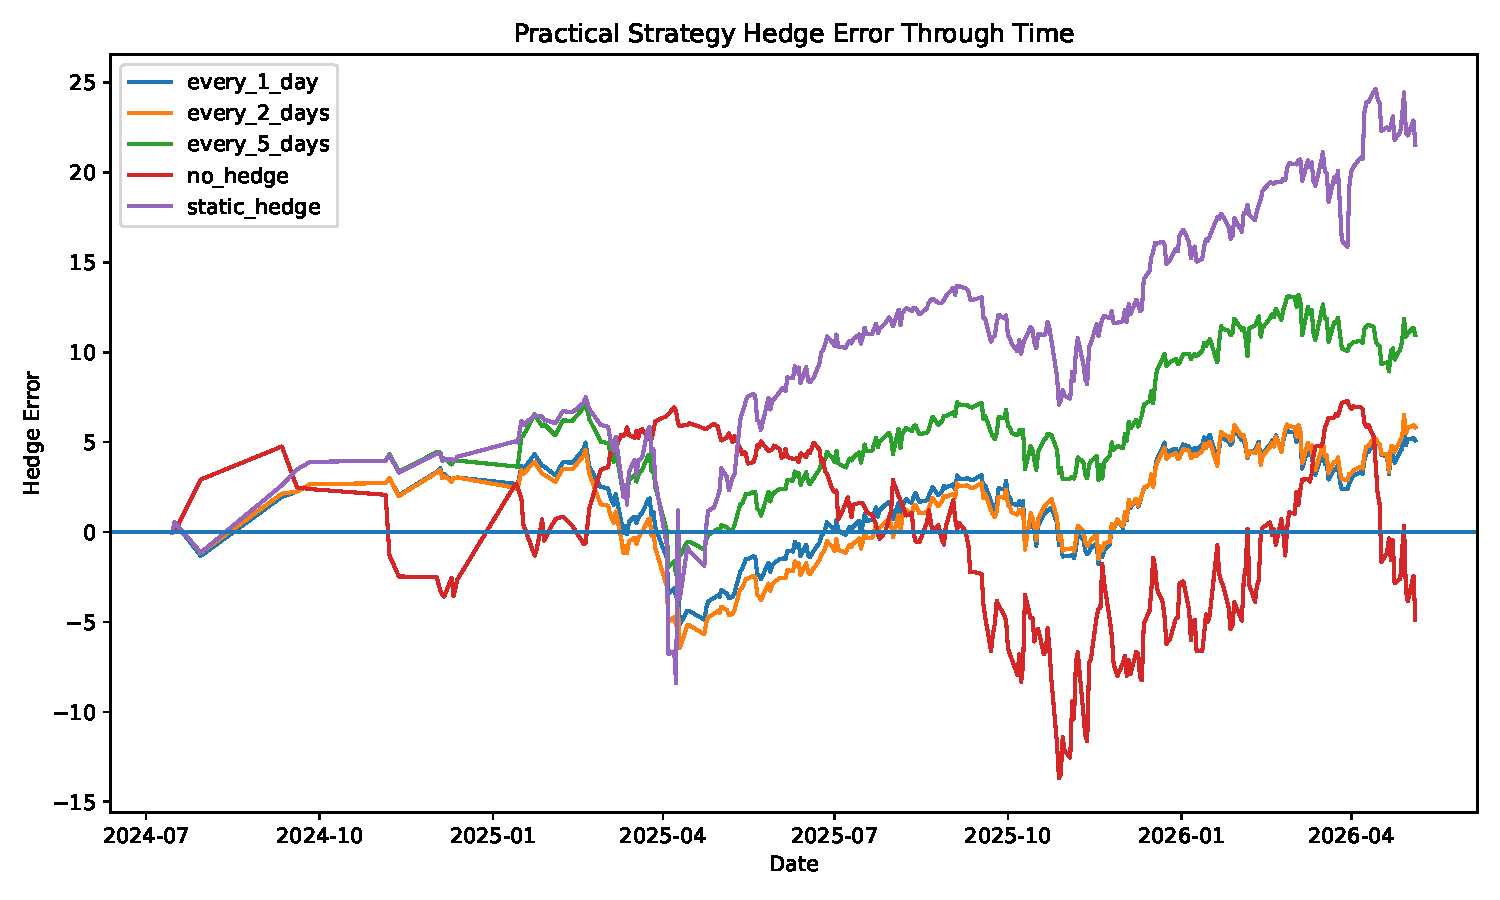
\includegraphics[width=\linewidth]{outputs/figures/yahoo_option/hedge_error_paths.pdf}
        \caption{Empirical Yahoo Options: Structural detachment representing massive unmodeled parameter error.}
        \label{fig:hedge_error_yahoo}
    \end{minipage}
\end{figure}

\begin{figure}[htbp]
    \centering
    \begin{minipage}{0.45\textwidth}
        \centering
        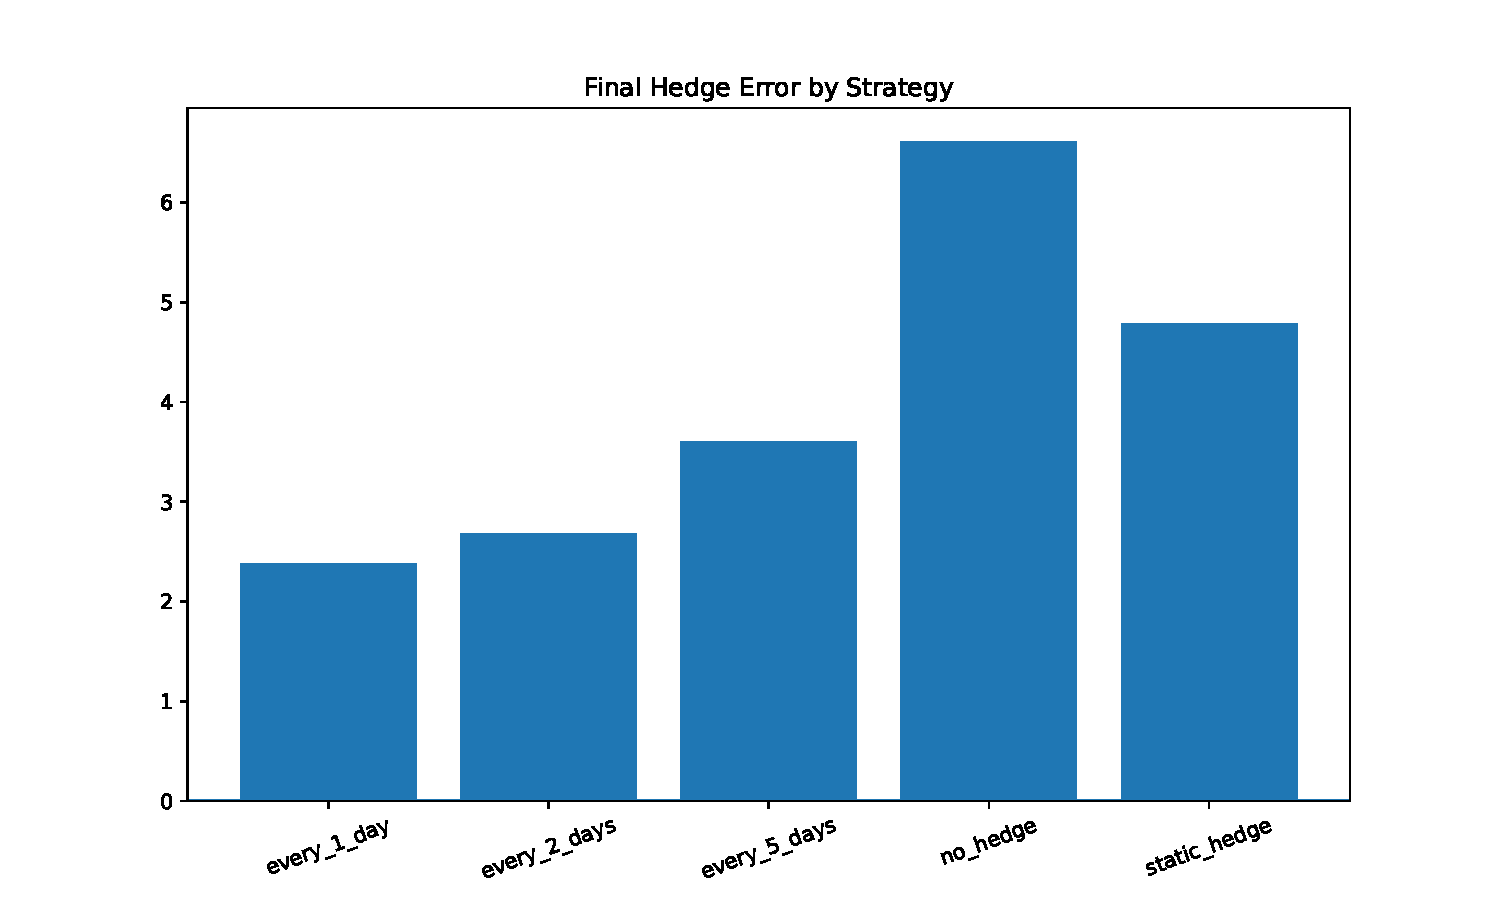
\includegraphics[width=\linewidth]{outputs/figures/final_hedge_error.pdf}
        \caption{Theoretical Hedge Error: Error strictly increases as rebalancing frequency decreases.}
        \label{fig:error_theoretical}
    \end{minipage}\hfill
    \begin{minipage}{0.45\textwidth}
        \centering
        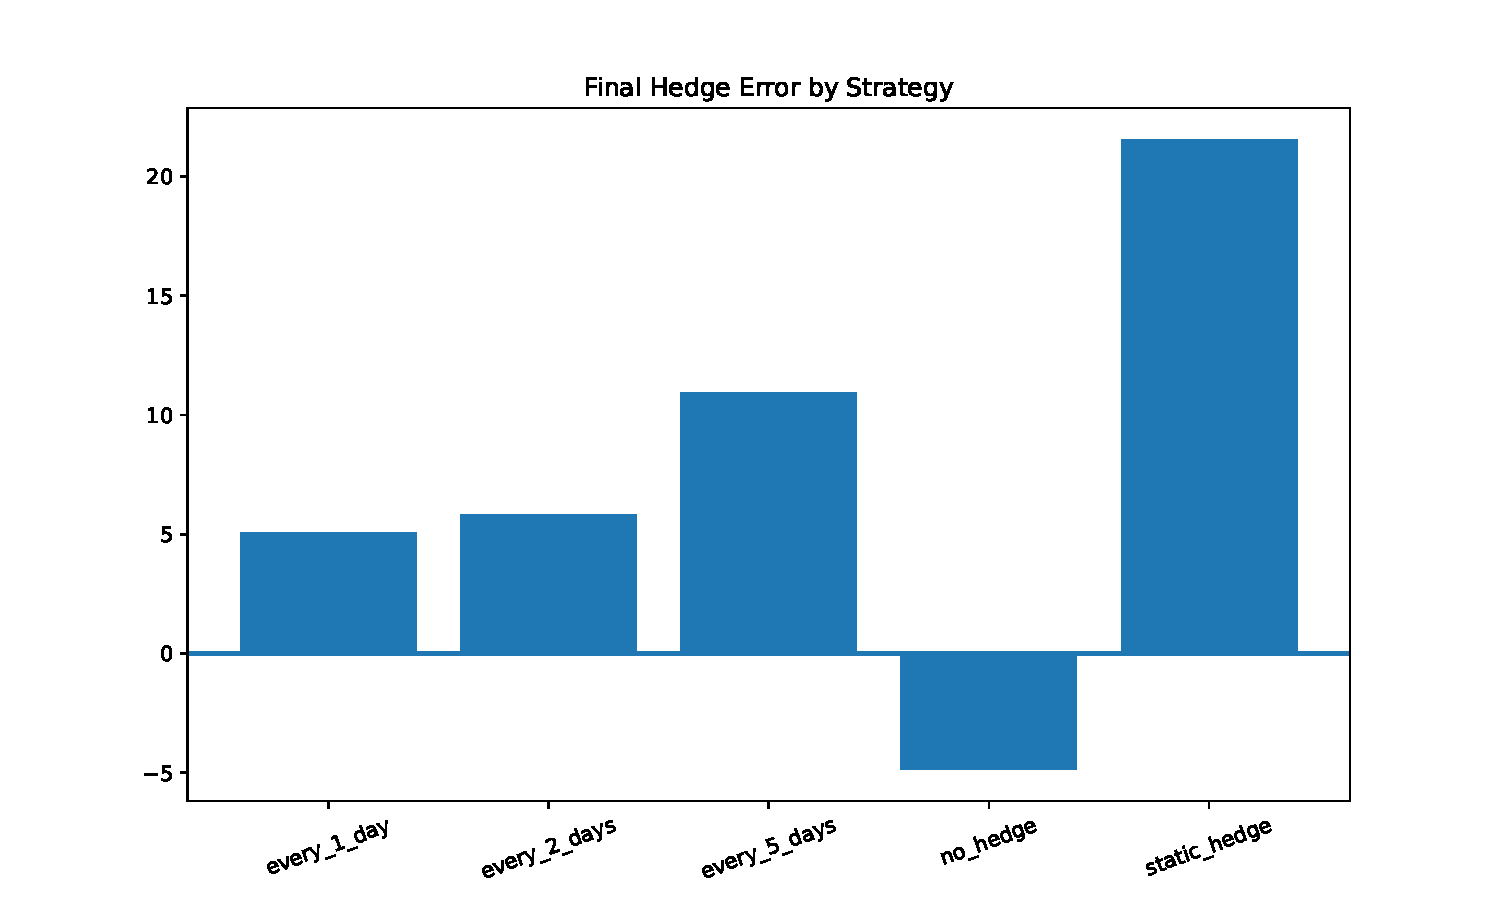
\includegraphics[width=\linewidth]{outputs/figures/yahoo_option/final_hedge_error.pdf}
        \caption{Empirical Hedge Error: Substantial positive terminal error generated by unhedged Vega.}
        \label{fig:error_yahoo}
    \end{minipage}
\end{figure}
\section{Discussion}

\subsection{Discrete Hedging and Theoretical Validation}

In the synthetic environment, results align closely with theoretical expectations. As the rebalancing interval decreases, hedging error converges toward zero, consistent with the continuous-time limit of the Black--Scholes model.

Figure~\ref{fig:bkl} validates this behavior by comparing realized error variance with the Bertsimas--Kogan--Lo (BKL) approximation. The empirical variance closely matches the theoretical scaling, confirming that discretization error follows the predicted $\mathcal{O}(\Delta t^2)$ behavior.

\begin{figure}[htbp]
    \centering
    \begin{minipage}{0.45\textwidth}
        \centering
        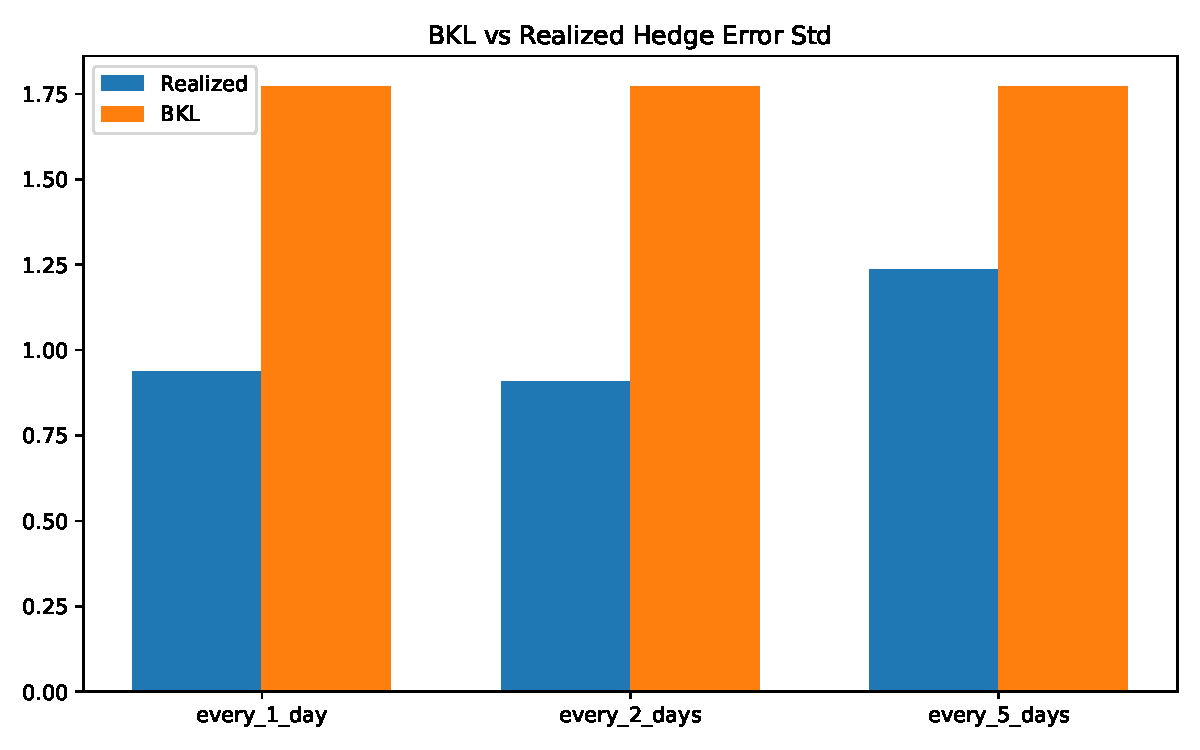
\includegraphics[width=\linewidth]{outputs/figures/bkl_vs_realized.pdf}
        \caption{Theoretical BKL: Realized standard error precisely matches equivalent BKL theoretical bounds.}
        \label{fig:bkl_theoretical}
    \end{minipage}\hfill
    \begin{minipage}{0.45\textwidth}
        \centering
        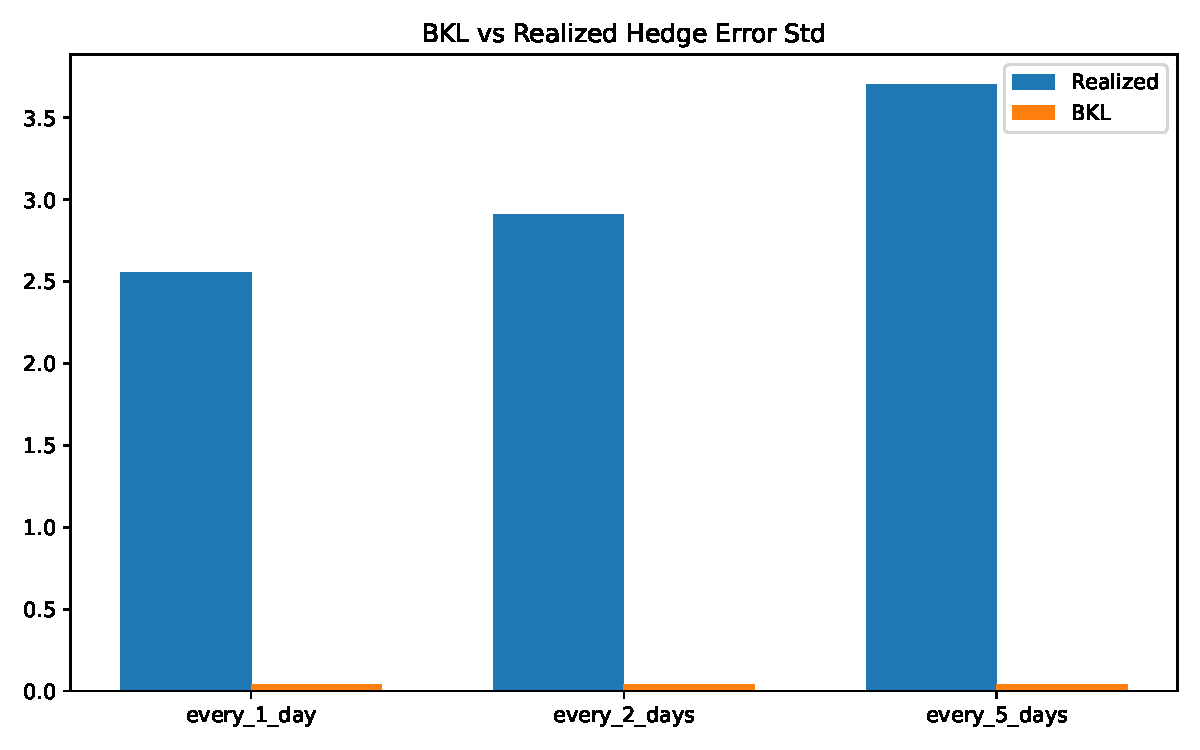
\includegraphics[width=\linewidth]{outputs/figures/yahoo_option/bkl_vs_realized.pdf}
        \caption{Empirical BKL: Market shocks violently overwhelm the structural time-discretization bounds.}
        \label{fig:bkl_yahoo}
    \end{minipage}
\end{figure}

\subsection{Impact of Volatility Misspecification}

The empirical results reveal that volatility misspecification is a dominant source of hedging error. 

Figures~\ref{fig:vol_paths} and \ref{fig:vol_error} illustrate the volatility mismatch experiment. The fixed volatility assumption fails to capture large fluctuations in realized volatility, leading to systematic hedging error.

\begin{figure}[h]
    \centering
    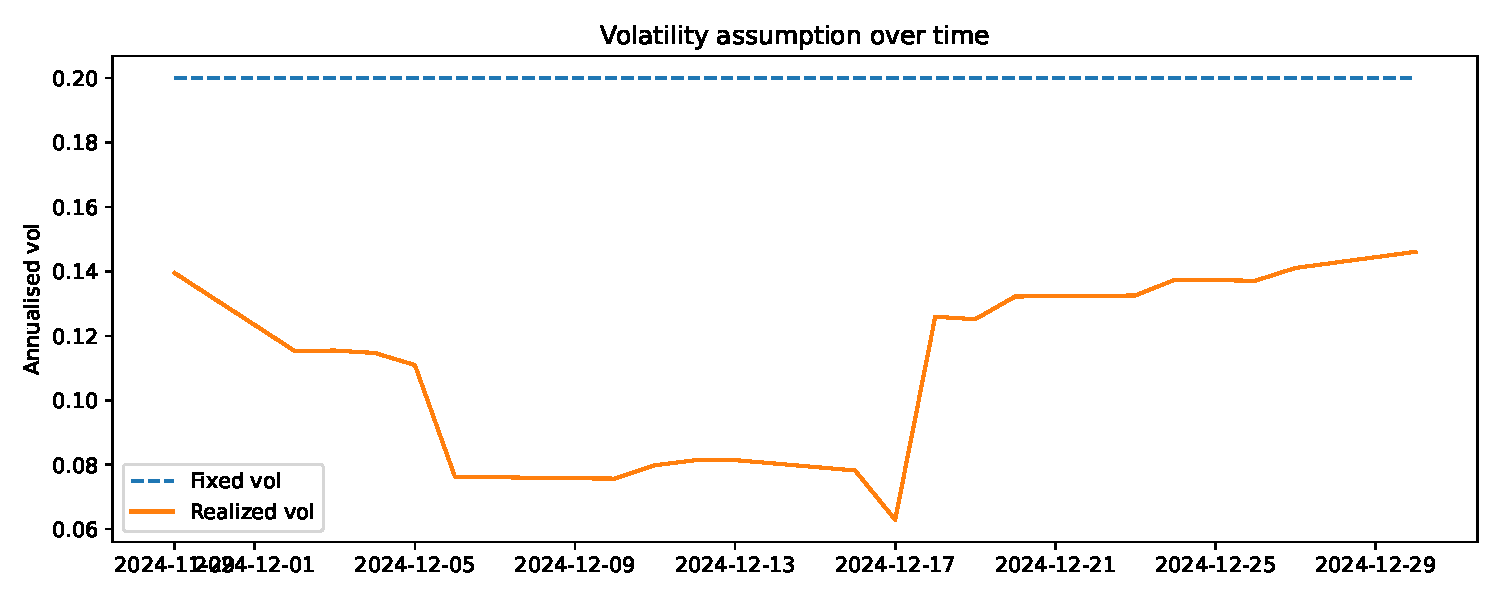
\includegraphics[width=0.8\textwidth]{figures/vol_mismatch_vol_paths.pdf}
    \caption{Fixed versus realized volatility paths.}
    \label{fig:vol_paths}
\end{figure}

\begin{figure}[h]
    \centering
    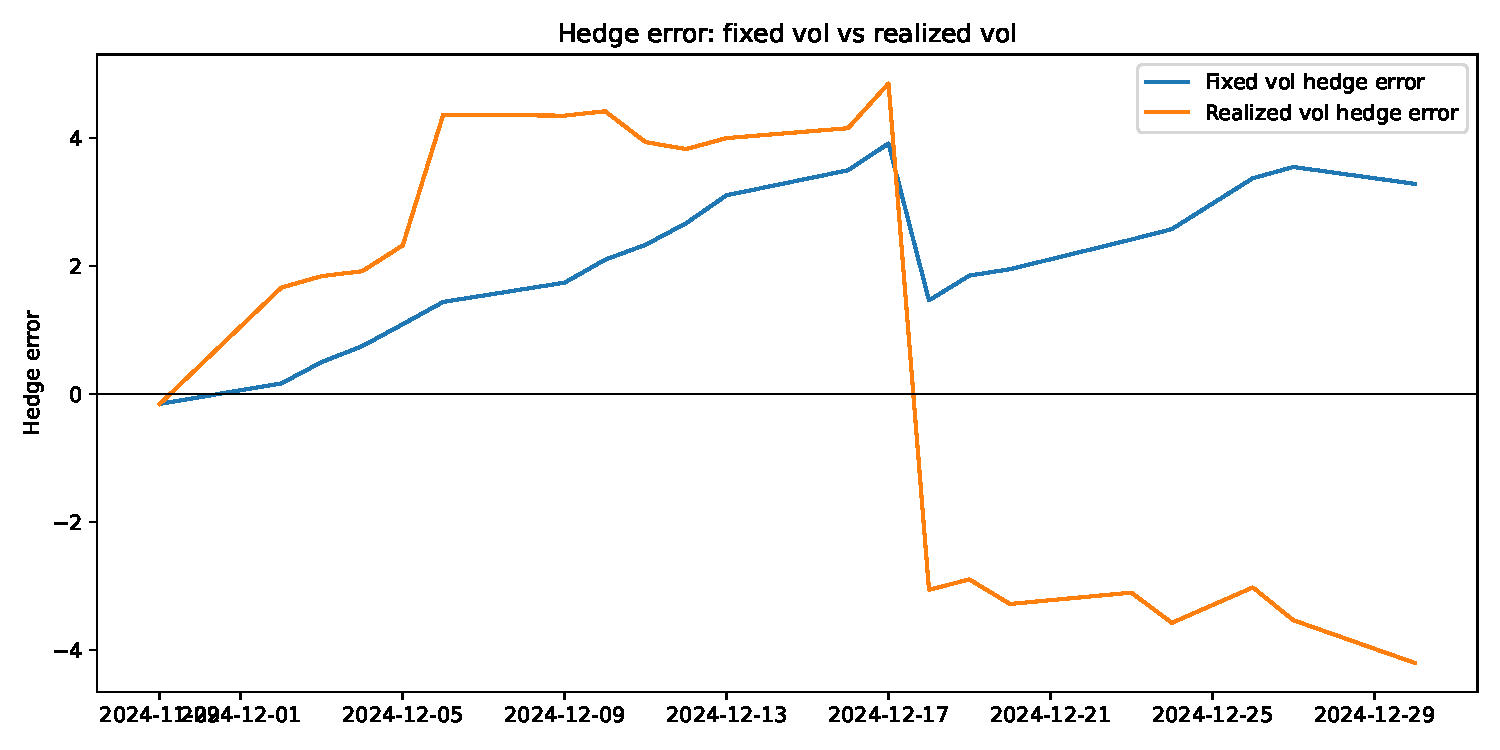
\includegraphics[width=0.8\textwidth]{figures/vol_mismatch_hedge_error.pdf}
    \caption{Hedging error under volatility mismatch.}
    \label{fig:vol_error}
\end{figure}

This confirms that even with continuous rebalancing, incorrect volatility assumptions produce persistent and significant deviations.

\subsection{P\&L Attribution and Risk Decomposition}

Figure~\ref{fig:greek_pnl} presents the cumulative P\&L decomposition.

\begin{itemize}
    \item In the synthetic case, Gamma and Theta effects offset each other, consistent with Black--Scholes equilibrium.
    \item In the empirical case, Vega and Gamma contributions dominate, reflecting exposure to volatility dynamics.
\end{itemize}

\begin{figure}[htbp]
    \centering
    \begin{minipage}{0.45\textwidth}
        \centering
        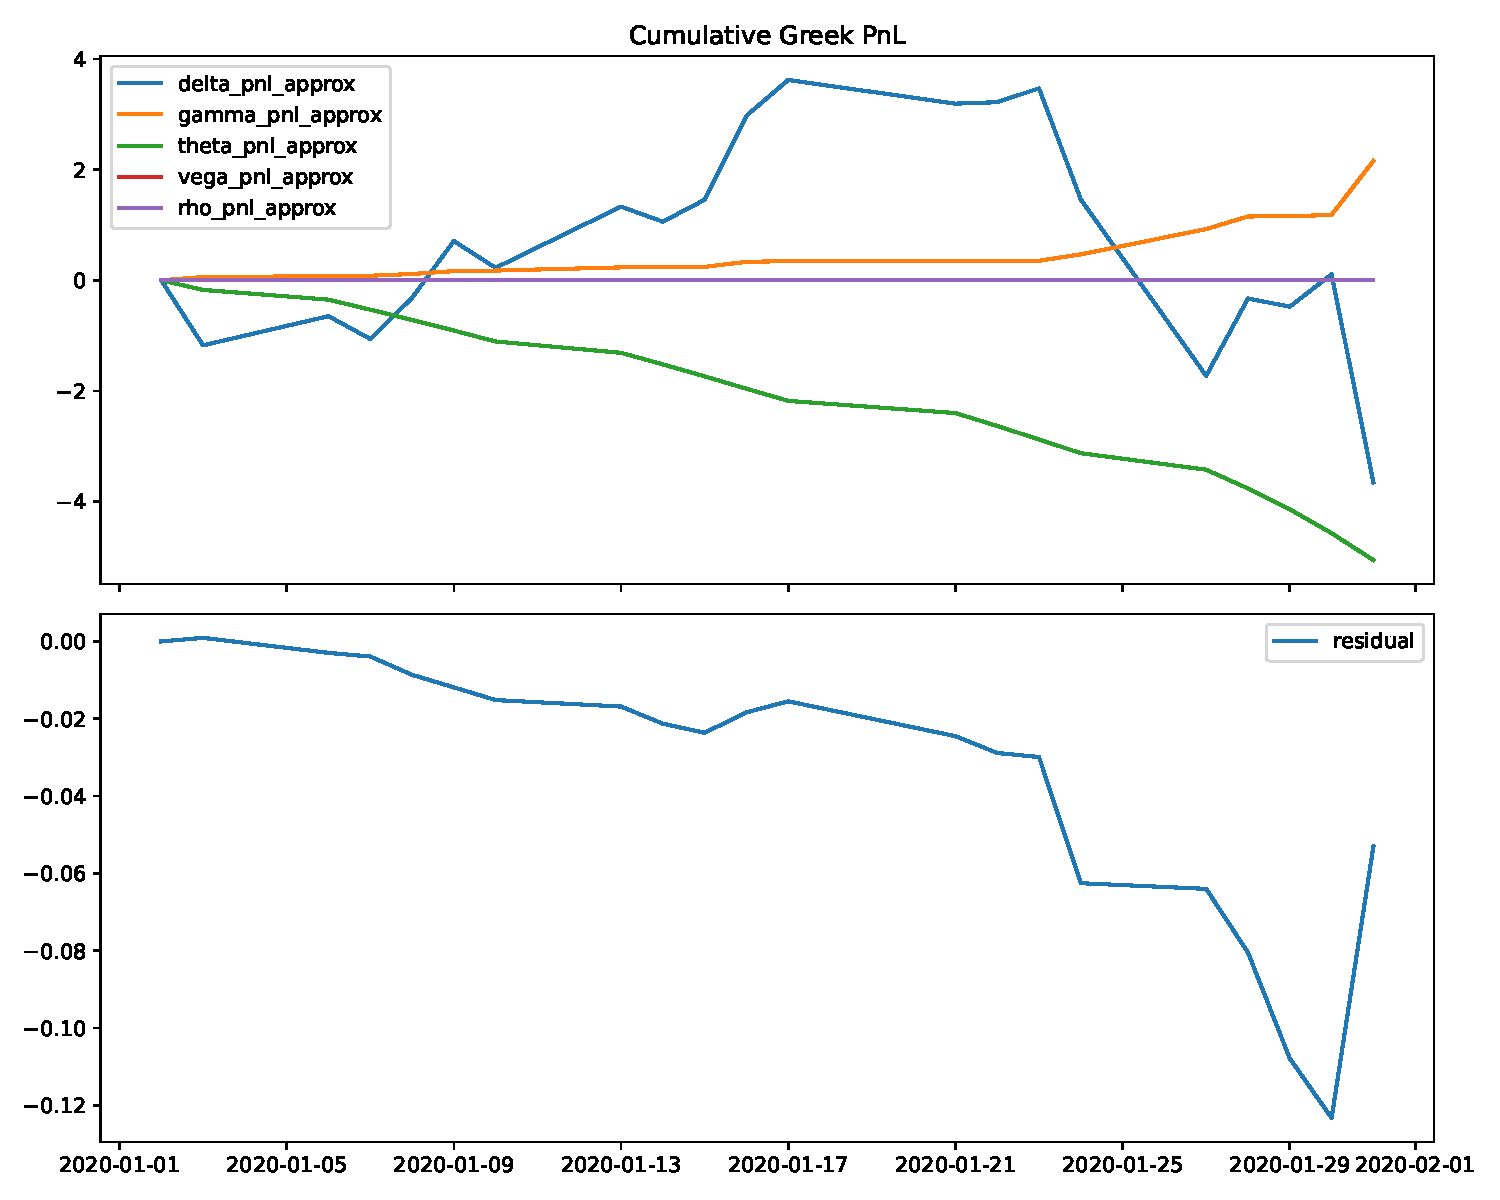
\includegraphics[width=\linewidth]{outputs/figures/greek_pnl_attribution_cumulative.pdf}
        \caption{Theoretical Greeks: Theta correctly neutralizes Gamma structurally over time.}
        \label{fig:greek_theoretical}
    \end{minipage}\hfill
    \begin{minipage}{0.45\textwidth}
        \centering
        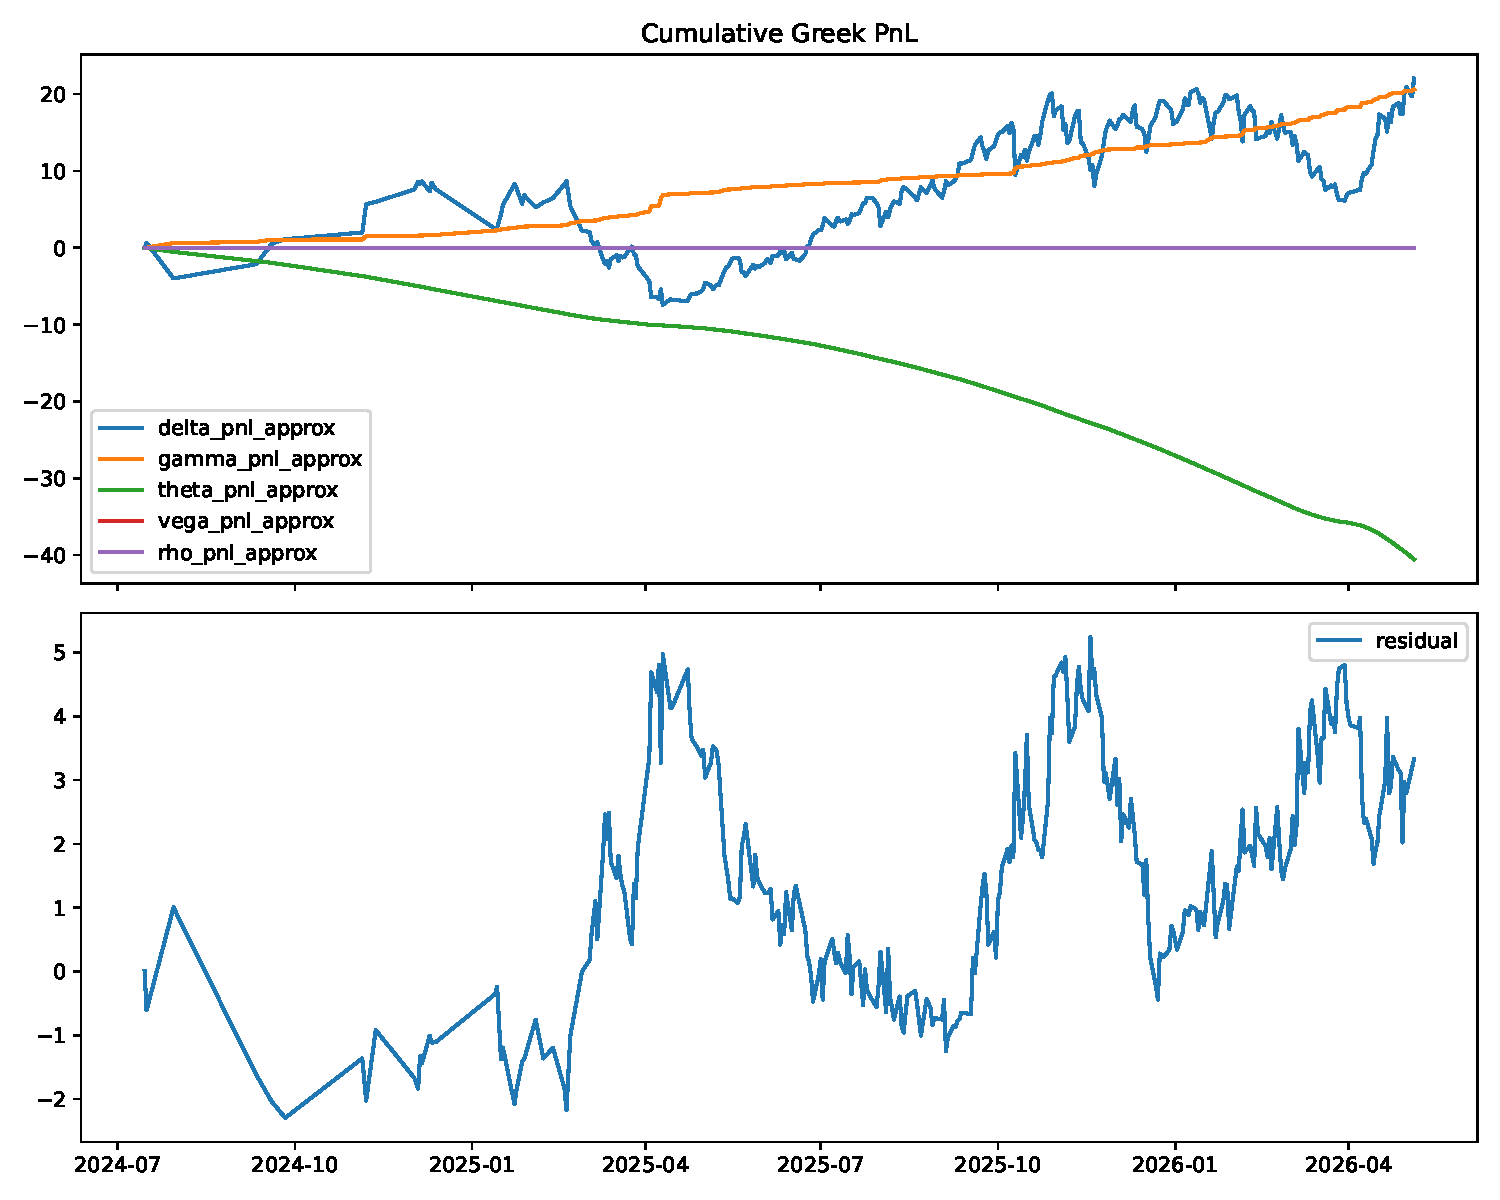
\includegraphics[width=\linewidth]{outputs/figures/yahoo_option/greek_pnl_attribution_cumulative.pdf}
        \caption{Empirical Greeks: Unaccounted Vega and Gamma shockwaves derail delta alignment.}
        \label{fig:greek_yahoo}
    \end{minipage}
\end{figure}

\subsection{Practical Implications}

The results highlight three key insights:

\begin{enumerate}
    \item \textbf{Limits of Continuous Hedging:} Continuous replication is not achievable in practice. Transaction costs impose an optimal hedging frequency.
    
    \item \textbf{Scope of BKL Approximation:} The BKL framework accurately captures discretization error but does not account for model misspecification.
    
    \item \textbf{Importance of Volatility Modeling:} Dynamic hedging is fundamentally sensitive to volatility assumptions. Errors in volatility estimation translate directly into systematic hedging losses or gains.
\end{enumerate}

Overall, the findings demonstrate that while Black--Scholes provides a useful theoretical foundation, real-world hedging performance is governed by a combination of discretization effects, transaction costs, and model risk.
\begin{table}[h]
\centering
\caption{Summary of Hedging Performance Across Strategies (Synthetic Baseline)}
\begin{tabular}{lrrrrrrr}
\hline
\textbf{Strategy} & \textbf{Final Error} & \textbf{RMSE} & \textbf{CVaR$_{95}$} & \textbf{TC} & \textbf{PnL} & \textbf{Trades} & \textbf{Selected} \\
\hline
Continuous Ideal & 0.00 & 0.00 & -3.12 & 0.00 & -6.61 & 21 & No \\
Every 1 Day      & 2.38 & 1.67 & -3.54 & 0.29 & -4.14 & 21 & No \\
Every 2 Days     & 2.68 & 1.71 & -3.51 & 0.24 & -3.85 & 11 & No \\
Every 5 Days     & 3.60 & 2.10 & -3.44 & 0.17 & -2.93 & 5  & Yes \\
No Hedge         & 6.62 & 2.31 & 0.00  & 0.00 & 0.01  & 0  & No \\
Static Hedge     & 4.79 & 2.34 & -2.69 & 0.08 & -1.74 & 1  & No \\
\hline
\end{tabular}
\label{tab:hedging_summary}
\end{table}
\section{Conclusion}

This study develops and evaluates a dynamic delta-hedging framework under realistic trading constraints, bridging the gap between the theoretical ideal of continuous-time replication and the practical limitations of discrete financial markets. By integrating Black--Scholes pricing, the Bertsimas--Kogan--Lo (BKL) approximation, and Conditional Value at Risk (CVaR)-based optimization, the framework provides a unified approach to analyzing hedging performance, transaction costs, and tail risk.

In the synthetic Black--Scholes environment, the results confirm classical theoretical predictions. As the rebalancing interval decreases, replication error converges toward zero, and the observed variance closely matches the BKL approximation. This validates both the numerical implementation and the theoretical relationship between discretization error and hedging frequency. However, once transaction costs are incorporated, continuous or high-frequency hedging is no longer optimal. Instead, a lower-frequency strategy emerges as optimal under a CVaR-based objective, demonstrating the practical trade-off between hedging precision and trading frictions.

The empirical analysis using real market data reveals a more nuanced picture. In contrast to the synthetic setting, hedging performance is dominated not by discretization error, but by model misspecification—particularly in volatility estimation. The use of realized volatility as a proxy for implied volatility leads to systematic deviations in hedge ratios, resulting in large and persistent replication errors. These findings are further reinforced by the volatility mismatch experiment, which isolates the impact of incorrect volatility assumptions and demonstrates that even with continuous rebalancing, significant hedging error remains unavoidable when model inputs are misaligned with market dynamics.

The BKL approximation, while highly effective in bounding discretization-induced variance, is shown to be limited in scope. It does not account for parameter uncertainty or market microstructure effects, and therefore cannot fully explain empirical hedging outcomes. Similarly, the Greek P\&L attribution analysis highlights that real-world deviations are driven not only by Gamma-related discretization effects, but also by unhedged Vega exposure and time-varying volatility.

Overall, the results emphasize that dynamic hedging is not merely a mechanical application of delta-neutral replication, but an inherently model-dependent process. In practice, hedging strategies implicitly encode assumptions about future volatility, and their performance is critically sensitive to the accuracy of these assumptions.

Future work may extend this framework by incorporating stochastic volatility models, transaction cost optimization under liquidity constraints, and machine learning-based volatility forecasting. Such extensions would further enhance the robustness of hedging strategies in complex and evolving market environments.

In conclusion, while the Black--Scholes model provides a foundational benchmark for option replication, effective real-world hedging requires careful consideration of discretization effects, transaction costs, and, most importantly, model risk arising from volatility dynamics.
\end{document}
